% !TeX spellcheck = da_DK
% Setup document class.
%  This will always be the beamer class, but depending on the use of notes,
%  it can be annotated with the option [notes] or  [notes=only], depending
%  on whether notes should be included, or should be the only thing in
%  the document.

\documentclass[xcolor=table]{beamer}

%%%% USE WHEN PRINING HANDOUTS %%%%%

%\documentclass[xcolor=table, handout]{beamer}
%\usepackage{pgfpages}
%\pgfpagesuselayout{2 on 1}[a4paper,border shrink=5mm]

%%%%%%%


% Setup theme.
%\usetheme[
%%% options passed to the outer theme
%    progressstyle=fixedCircCnt,   %either fixedCircCnt, movCircCnt, or corner
%    rotationcw,          % change the rotation direction from counter-clockwise to clockwise
%    shownavsym          % show the navigation symbols
]{AAUsimple}

\usetheme[
%%% options passed to the outer theme
%    hidetitle,           % hide the (short) title in the sidebar
%    hideauthor,          % hide the (short) author in the sidebar
%    hideinstitute,       % hide the (short) institute in the bottom of the sidebar
%    shownavsym,          % show the navigation symbols
%    width=2cm,           % width of the sidebar (default is 2 cm)
    hideothersubsections,% hide all subsections but the subsections in the current section
%    hideallsubsections,  % hide all subsections
    left              % right of left position of sidebar (default is right)
%%% options passed to the color theme
%    lightheaderbg,       % use a light header background
  ]{AAUsidebar}

\setbeamercolor{alerted text}{fg=blue,bg=}


% Import preamble
%%% Initial things %%%
% Increase number of dimen registers
\usepackage{etex}
% Fix various issues with LaTeX2e
\usepackage{fixltx2e}
% Font package
\usepackage{fourier}


%%% Translations and character encodings %%%
% Enable use of several characters, including æ, ø and å
\usepackage[utf8]{inputenc}
% Danish language
\usepackage[UKenglish]{babel}
% Use PostScript fonts instead of bitmap ones. Also does other stuff.
\usepackage[T1]{fontenc}
% Various LaTeX symbols
\usepackage{latexsym}
% Wider selection of colours
\usepackage{xcolor}
% Improved element justification
\usepackage{ragged2e}
% Font improvements
\usepackage{fix-cm}
% Enables various forms of lines, like double-underlining (\uuline{})
\usepackage{ulem}
% Sets the tolerance for distance between words, determining when to hyphenate.
\pretolerance=2500

\usepackage{rotating}

%%% Figures and tables (Floats) %%%
% Enable multi-rows and -columns
\usepackage{multirow}
\usepackage{multicol}
% Double, horizontal lines
\usepackage{hhline}
% Enables coloured tables
\usepackage{colortbl}
% Prettier tables
\usepackage{booktabs}


%%% Mathematic formulas %%%
% AMS math
\usepackage{amsmath}
\usepackage{amssymb}
% Extra fonts (for math, I think)
\usepackage{stmaryrd}
% Access text symbols
\usepackage{textcomp}
% Extend AMS
\usepackage{mathtools}
\usepackage{cancel}


%%% Graphics %%%
% Various image-commands
\usepackage{eso-pic}
% Use JPEG and PNG images
\usepackage{graphicx}

%%% Code listing %%%
\usepackage{color}
\definecolor{bluekeywords}{rgb}{0.13,0.13,1}
\definecolor{greencomments}{rgb}{0,0.5,0}
\definecolor{redstrings}{rgb}{0.9,0,0}

\usepackage{courier}

\usepackage{listings}

\lstset{language=[Sharp]C,
  captionpos=b,
  columns=fixed,
  numbers=left,
  numberstyle=\tiny,
  showspaces=false,
  showtabs=false,
  tabsize=3,
  breaklines=true,
  inputencoding=utf8,
  showstringspaces=false,
  breakatwhitespace=true,
  escapeinside={(*@}{@*)},
  commentstyle=\color{greencomments},
  keywordstyle=\color{bluekeywords},
  stringstyle=\color{redstrings},
  basicstyle=\ttfamily\small,
}

\lstdefinestyle{make}{tabsize=2}


%%% References, bibtex and URLs %%%
% Post URLs. Allows breaking at hyphens to help avoid long links.
\usepackage{url}
% Better cross references
\usepackage[english]{varioref}
% Define a new 'leo' style for URL package, that will use a smaller font
\makeatletter
\def\url@leostyle{%
  \@ifundefined{selectfont}{\def\UrlFont{\sf}}{\def\UrlFont{\small\ttfamily}}
}
\makeatother
% And of course, use this new style
\urlstyle{leo}

\hypersetup{pdfstartview={Fit}}
%%%%%%%%%%%%%%%%%%%%%%%%%%%%%%%%%%%%%%%%%%%%%%%%
%Flowchart
\usepackage{tikz}
\usepackage{tkz-graph}
\usetikzlibrary{shapes,arrows}
\usepackage{tikz-qtree}
\usepackage{tikzscale}
\usetikzlibrary{shapes.multipart, arrows, matrix, automata, positioning, shadows, decorations.pathreplacing, calc}
%%%%%%%%%%%%%%%%%%%%%%%%%%%%%%%%%%%%%%%%%%%%%%%%



\usepackage{color}
\definecolor{bluekeywords}{rgb}{0.13,0.13,1}
\definecolor{greencomments}{rgb}{0,0.5,0}
\definecolor{redstrings}{rgb}{0.9,0,0}
\usepackage{courier}
\usepackage{listings}

\lstset{
    literate={ø}{{\o}}1
         {æ}{{\ae}}1
         {å}{{\aa}}1
         {Ø}{{\O}}1
         {Æ}{{\AE}}1
         {Å}{{\AA}}1
         {§}{{\S}}1
}

%%% Colour definitions %%%
% Defines: gray
\definecolor{gray}{gray}{0.80}
% Defines: numbercolor
\definecolor{numbercolor}{gray}{0.7}
% Defines: shadecolor
\definecolor{shadecolor}{RGB}{33,26,82}
% Defines: aaublue

\definecolor{aaublue}{RGB}{33,26,82}


\colorlet{punct}{red!60!black}
\definecolor{background}{HTML}{EEEEEE}
\definecolor{delim}{RGB}{20,105,176}
\colorlet{numb}{magenta!60!black}

\newcommand*\rot{\rotatebox{90}}


\usepackage{pifont}
\newcommand{\cmark}{\ding{51}}%
\newcommand{\xmark}{\ding{55}}%

\usepackage{todonotes}


\showboxdepth=5
\showboxbreadth=5


\tikzstyle{decision} = [diamond, draw, fill=yellow!20, text width=4.5em, text badly centered, node distance=3cm, inner sep=3pt]
\tikzstyle{block} = [rectangle, draw, fill=green!40, text width=5em, text centered, rounded corners, minimum height=4em]
\tikzstyle{line} = [draw, -latex']
%\tikzstyle{cloud} = [draw, ellipse,fill=red!20, node distance=3cm, minimum height=2em]
\tikzstyle{cloud_nospace} = [cloud, node distance=1cm]
\tikzstyle{preDefProc} = [draw,rectangle split, rectangle split horizontal,rectangle split parts=3, fill=green!40,minimum height=4em]


\definecolor{OliveGreen}{rgb}{0,0.6,0}
\definecolor{aaublue}{RGB}{33,26,82}
\definecolor{wiki_important}{HTML}{F4DDDB}
\definecolor{wiki_important_text}{HTML}{464C5C}
\definecolor{wiki_important_line}{HTML}{C0392B}
%Google colors from https://www.google.com/design/spec/style/color.html#color-color-palette
\definecolor{GoogleRed}{HTML}{F44336}
\definecolor{GooglePurple}{HTML}{9C27B0}
\definecolor{GoogleDeepPurple}{HTML}{673AB7}
\definecolor{GoogleIndigo}{HTML}{3F51B5}   
\definecolor{GoogleBlue}{HTML}{2196F3}   
\definecolor{GoogleLightBlue}{HTML}{03A9F4}   
\definecolor{GoogleCyan}{HTML}{00BCD4}   
\definecolor{GoogleTeal}{HTML}{009688}   
\definecolor{GoogleGreen}{HTML}{4CAF50}
\definecolor{GoogleLightGreen}{HTML}{8BC34A}
\definecolor{GoogleLime}{HTML}{CDDC39}
\definecolor{GoogleYellow}{HTML}{FFEB3B}
\definecolor{GoogleAmber}{HTML}{FFC107}
\definecolor{GoogleOrange}{HTML}{FF9800}
\definecolor{GoogleDeepOrange}{HTML}{FF5722}
\definecolor{GoogleBrown}{HTML}{795548}
\definecolor{GoogleGrey}{HTML}{9E9E9E}
\definecolor{GoogleBlueGrey}{HTML}{607D8B}   


\usepackage{csquotes}


% Additional settings for boxes
\setbeamercolor{headerCol}{fg=black,bg=lightgray}
\setbeamercolor{bodyCol}{fg=white,bg=gray}
\setbeamercovered{transparent=20}

% Define document stuff
\title[GIRAF]{Software Development in the GIRAF Multi–Project}
\subtitle[Exam]{Exam Presentation}
\author[SW618F16]{SW618F16}
\date{June 20th 2016}

\institute[
%  {\includegraphics[scale=0.2]{aau_segl}}\\ %insert a company, department or university logo
Software (SW6)\\
Aalborg University\\
Denmark
] % optional - is placed in the bottom of the sidebar on every slide
{% is placed on the title page
  Aalborg University\\
  Denmark

  %there must be an empty line above this line - otherwise some unwanted space is added between the university and the country (I do not know why;( )
}

% Specify a logo on the titlepage (you can specify additional logos an include them in
% institute command below
\pgfdeclareimage[height=1.5cm]{titlepagelogo}{AAUgraphics/aau_logo_new} % placed on the title page
%\pgfdeclareimage[height=1.5cm]{titlepagelogo2}{graphics/aau_logo_new} % placed on the title page
\titlegraphic{% is placed on the bottom of the title page
  \pgfuseimage{titlepagelogo}
  %  \hspace{1cm}\pgfuseimage{titlepagelogo2}
}


\begin{document}

{\aauwavesbg
  \begin{frame}[plain,noframenumbering]
    \titlepage
  \end{frame}}

% ==================== SUBJECTS ======================
\section{Introduction}
    \begin{frame}[t]{Introduction}\framesubtitle{The Multi--Project}
        \begin{itemize}
	        \item What is GIRAF?
	        	\begin{itemize}
	        		\item \textbf{G}raphical \textbf{I}nterface \textbf{R}esources for \textbf{A}utistic \textbf{F}olk
	        	\end{itemize}
        	\item Bachelor project started 6 years ago
        	\item Multiple Team Software Development
        	\item Minimal Viable Product
        		\begin{itemize}
        			\item Launcher 
        			\item Week Schedule and its prerequisites
        			\item Voice Game as stand--alone
        		\end{itemize}
    			\item No synchronisation
    			\item No security
    		\end{itemize}
    \end{frame}

\section{Development Processes}
	\subsection{Description}
	\subsubsection{Multi--Project}
    \begin{frame}[t]{Development Process}\framesubtitle{Cooperating in multiple teams}
    \begin{itemize}
        \item Scrum of Scrums
        	\begin{itemize}
        		\item Weekly meeting
    			\begin{itemize}
        			\item Knowledge sharing 
        			\item Help seeking
        		\end{itemize}
        		\item Product Owner        			
    			\begin{itemize}
        			\item Important role
        			\item Not everyone in the group participated
        			\item Problems within their groups
        			\item Weak communication with customers
        			\item User stories
        		\end{itemize}
        		\item Scrum Master
        		\begin{itemize}
        			\item Wanted to be PO themselves
        			\item Helped when the PO needed help
        		\end{itemize}
    		\end{itemize}
    \end{itemize}
	\end{frame}
	 \subsubsection{Internal--Project}
	\begin{frame}[t]{Development Process}\framesubtitle{Internal Process}
    \begin{itemize}
        \item Scrum
        \begin{itemize}
        	\item Daily Scrum
        	\item Scrumboard
        \end{itemize}
        \item Pair Programming
        \bigskip
        \item Improved the use of these over time
    \end{itemize}
	\end{frame}
	\subsubsection{Rest--API Project}
		\begin{frame}[t]{Development Process}\framesubtitle{REST API}
	
    \begin{itemize}
        \item Close cooperation between two groups
        \item High code quality
        \item Should be easy to continue work on
        \item Stricter code review
        \item Well thought out design
        \item Automatic integration tests
    \end{itemize}
	\end{frame}

	\subsection{Evaluation}
		\begin{frame}[t]{Evaluation}\framesubtitle{Evaluating the processes}
	
    \begin{itemize}
        \item Sprint Retrospectives
        \item Development process underwent changes we wanted
        \begin{itemize}
        	\item User Stories
        	\item Sub-tasks for user stories
        \end{itemize}
        \item Our own thoughts
        	\begin{itemize}
        		\item A \textit{Co--ordinator} of each app
        		\item Groups working on the same app should have better communication
        	\end{itemize}
    \end{itemize}
	\end{frame}
\section{Project Management \& Development}
\subsection{Obstacles}
\begin{frame}{Project Management \& Development}
    \begin{itemize}
        \item Version Control
        \begin{itemize}
            \item Manageing repositories and sourcecode
        \end{itemize}
        \item Code Review
        \item Wiki
        \item Documentation
        \item Continuous Integration
        \item Artifact Repository
    \end{itemize}
\end{frame}
\subsection{Tools}
\begin{frame}[t]{Project Management \& Development}\framesubtitle{Version Control}
    \begin{itemize}
        \item Git
        \begin{itemize}
            \item Foundation of the workflow
            \item Gogs
            \begin{itemize}
                \item Restricted to AAU developers
                \item Custom git--hooks
            \end{itemize}
            \item Powerful
            \item Easy to make mistakes
        \end{itemize}
    \end{itemize}
\end{frame}

\begin{frame}[t]{Project Management \& Development}\framesubtitle{Code Review, Wiki}
    \begin{itemize}
        \item Phabricator
        \begin{itemize}
            \item Arcanist
            \begin{itemize}
                \item Uses git
                \item Interfaces with Phabricator
                \item Unit tests \& linting
            \end{itemize}
            \item Web interface
            \begin{itemize}
                \item Hub for the entire multi--project
                \item User story and task management
                \begin{itemize}
                    \item Backlog
                    \item Assign to groups
                \end{itemize}
                \item Scrumboards
                \item Wiki
                \item Code review
            \end{itemize}
        \end{itemize}
    \end{itemize}
\end{frame}
\begin{frame}[t]{Project Management \& Development}\framesubtitle{CI, Documentation, Artifact Repo}
    \begin{itemize}
        \item Jenkins
        \begin{itemize}
            \item Gradle
            \begin{itemize}
                \item DevOps
            \end{itemize}
            \item Automated Testing
            \begin{itemize}
                \item Monkey test
                \item Unit tests
            \end{itemize}
            \item Artifactory
            \begin{itemize}
                \item Maven repository
                \item Multiple versions of libraries
            \end{itemize}
            \item Javadoc
        \end{itemize}
    \end{itemize}
\end{frame}
\section{Architecture}
\begin{frame}[t]{Architecture}\framesubtitle{Old GIRAF architecture}
    \only<1>{%
    \begin{figure}
        \centering
        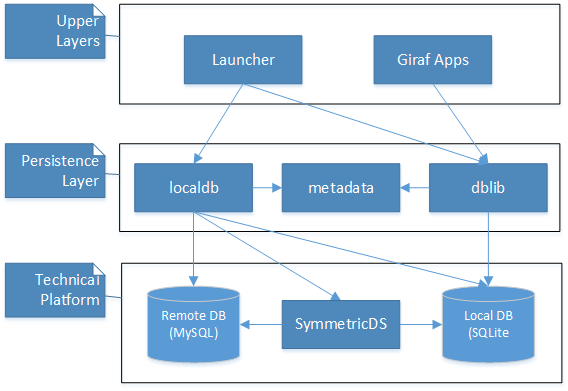
\includegraphics[width=0.8\textwidth]{images/old_architecture.png}
    \end{figure}}
    \only<2>{%
    \begin{figure}
        \centering
        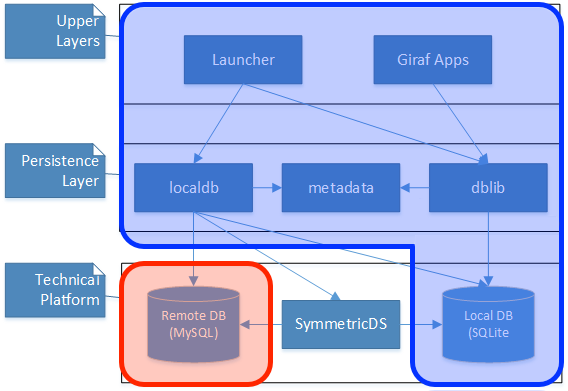
\includegraphics[width=0.8\textwidth]{images/old_architecture_memes.png}
    \end{figure}}
\end{frame}

\begin{frame}[t]{Architecture}\framesubtitle{New GIRAF architecture}
    \centering
    \scalebox{0.6}{%
    \pgfdeclarelayer{background}
\pgfsetlayers{background,main}
\tikzstyle{double_arrow}=[latex'-latex']
\tikzstyle{component}=[draw, fill=blue!20, text width=8em,
text centered, minimum height=2.5em]
\tikzstyle{client_comp}=[draw, fill=blue!20, text width=4em,
text centered, minimum height=2.5em]
\tikzstyle{client_comp_synca}=[draw, fill=blue!20, text width=4em,
text centered, minimum height=1.5em]
\tikzstyle{bgbox}=[fill=green!20, rounded corners, draw=GoogleGrey, dashed]
\begin{tikzpicture}[auto]

    %%%%%%%%%%%%%%%%%%%%%%%%%%%%%%%%%%%%%%%%%%%%%%%%%%%%%%%%%%%%%%%%%%%%%
    % REST API                                                          %
    %%%%%%%%%%%%%%%%%%%%%%%%%%%%%%%%%%%%%%%%%%%%%%%%%%%%%%%%%%%%%%%%%%%%%
    \node[component] (persistence) {Persistence};
    \node[component, above = 0.6cm of persistence] (service) {Service};
    %core
    \path (persistence.south -| persistence.east)+(1,0) node (core_a) {};
    \path (service.north -| service.east)+(2,0) node (core_b) {};
    \path[draw, fill = blue!20] (core_a) rectangle (core_b);
    \path ($ (core_a) !.5! (core_b) $) node (core) {Core};

    %REST API background box
    \begin{pgfonlayer}{background}
        % Compute a few helper coordinates
        \path (service.west |- service.north)+(-3,+0.5) node (rest_a) {};
        \path (core_a)+(+2,-0.5) node (rest_b) {};
        \path [bgbox] (rest_a) rectangle (rest_b);
        \node [below = 0.5em of rest_a, anchor = west, inner sep = 0.5em]{REST API};
    \end{pgfonlayer}

    %Awwowwwws
    \draw [<-, dashed] ($(service.south)+(+0.1,0)$) -- ($(persistence.north)+(+0.1,0)$);
    \draw [->]     ($(service.south)+(-0.1,0)$) -- ($(persistence.north)+(-0.1,0)$);
    \draw [->]     (service) -- node {uses} (service -| core_a);
    \draw [->]     (persistence) -- node {uses} (persistence -| core_a);

    %%%%%%%%%%%%%%%%%%%%%%%%%%%%%%%%%%%%%%%%%%%%%%%%%%%%%%%%%%%%%%%%%%%%%
    % Storage                                                           %
    %%%%%%%%%%%%%%%%%%%%%%%%%%%%%%%%%%%%%%%%%%%%%%%%%%%%%%%%%%%%%%%%%%%%%
    \node[component, below = 1.5cm of persistence] (db) {Database};

    \draw [<-, dashed] ($(persistence.south)+(+0.1,0)$) -- ($(db.north)+(+0.1,0)$);
    \draw [->]     ($(persistence.south)+(-0.1,0)$) -- ($(db.north)+(-0.1,0)$);

    %storage background box
    \begin{pgfonlayer}{background}
        % Compute a few helper coordinates
        \path (db.west |- db.north)+(-3,+0.5) node (db_a) {};
        \path (core_a |- db.south)+(+2,-0.5) node (db_b) {};
        \path [bgbox] (db_a) rectangle (db_b);
        \node [below = 0.5em of db_a, anchor = west, inner sep = 0.5em]{Storage};
    \end{pgfonlayer}

    %%%%%%%%%%%%%%%%%%%%%%%%%%%%%%%%%%%%%%%%%%%%%%%%%%%%%%%%%%%%%%%%%%%%%
    % Web 'n' client                                                    %
    %%%%%%%%%%%%%%%%%%%%%%%%%%%%%%%%%%%%%%%%%%%%%%%%%%%%%%%%%%%%%%%%%%%%%
    \node[draw, cloud, cloud puffs=12, cloud ignores aspect, minimum width=9em, minimum height=5em,fill=blue!20, above = 1cm of service](web) {Internet};
    \draw [<-, dashed] ($(web.south)+(+0.1,0)$) -- ($(service.north)+(+0.1,0)$);
    \draw [->]     ($(web.south)+(-0.1,0)$) -- ($(service.north)+(-0.1,0)$);

    % CLIENT GALORE
    \node[client_comp, above = 2cm of web](client2) {$\text{App}_{2}$};
    \node[client_comp_synca, below = 0.3cm of client2] (client2_synca) {S.A.};
    \draw [<-, dashed] ($(client2.south)+(+0.1,0)$) -- ($(client2_synca.north)+(+0.1,0)$);
    \draw [->]     ($(client2.south)+(-0.1,0)$) -- ($(client2_synca.north)+(-0.1,0)$);
    \draw [<-, dashed] ($(client2_synca.south)+(+0.1,0)$) -- ($(web.north)+(+0.1,0)$);
    \draw [->]     ($(client2_synca.south)+(-0.1,0)$) -- ($(web.north)+(-0.1,0)$);

    \node[client_comp, left = 0.2cm of client2](client1) {$\text{App}_{1}$};
    \node[client_comp_synca, below = 0.3cm of client1] (client1_synca) {S.A.};
    \draw [<-, dashed] ($(client1.south)+(+0.1,0)$) -- ($(client1_synca.north)+(+0.1,0)$);
    \draw [->]     ($(client1.south)+(-0.1,0)$) -- ($(client1_synca.north)+(-0.1,0)$);
    \draw [<-, dashed] ($(client1_synca.south)+(+0.1,0)$) |- ($(web.west)+(0,+0.1)$);
    \draw [->]     ($(client1_synca.south)+(-0.1,0)$) |- ($(web.west)+(0,-0.1)$);

    \node[right = 0.2cm of client2] (client_dot){$\cdots$};

    \node[client_comp, right = 0.2cm of client_dot](clientn) {$\text{App}_{n}$};
    \node[client_comp_synca, below = 0.3cm of clientn] (clientn_synca) {S.A.};
    \draw [<-, dashed] ($(clientn.south)+(+0.1,0)$) -- ($(clientn_synca.north)+(+0.1,0)$);
    \draw [->]     ($(clientn.south)+(-0.1,0)$) -- ($(clientn_synca.north)+(-0.1,0)$);
    \draw [<-, dashed] ($(clientn_synca.south)+(+0.1,0)$) |- ($(web.east)+(0,-0.1)$);
    \draw [->]     ($(clientn_synca.south)+(-0.1,0)$) |- ($(web.east)+(0,+0.1)$);

    %clients background box
    \begin{pgfonlayer}{background}
        % Compute a few helper coordinates
        \path (service.west |- client1.north)+(-3,+0.5) node (clients_a) {};
        \path (core_a |- clientn_synca.south)+(+2,-0.5) node (clients_b) {};
        \path[bgbox] (clients_a) rectangle (clients_b);
        \node [below = 0.5em of clients_a, anchor = west, inner sep = 0.5em]{Clients};
    \end{pgfonlayer}

\end{tikzpicture}
}
\end{frame}

\begin{frame}[t]{Architecture}\framesubtitle{New GIRAF architecture}
    \begin{itemize}
        \item Layered architecture
        \item Easier to test
        \item Scaleable
        \item Easier to make other GIRAF clients
    \end{itemize}
\end{frame}

\section{Products}
    \subsection{REST API}
        \begin{frame}[t]{Developing the REST API}\framesubtitle{Overview}
            \begin{itemize}
                \item Focus on the next generation of GIRAF developers
                \begin{itemize}
                    \item Documentation
                    \item Design
                \end{itemize}
                \item Synchronisation
                \item Security
            \end{itemize}
        \end{frame}

        \begin{frame}[t]{Developing the REST API}\framesubtitle{Our contributions}
            Sprints 3-4:
            \begin{itemize}
                \item Pictograms
                \item Sequences
                \item Week Schedules
            \end{itemize}
            \bigskip
            Differences from developing Apps.
            \begin{itemize}
                \item Unit Tests
                \item Linting
                \begin{itemize}
                    \item Saved time during code--review
                    \item Enforced a code--style
                \end{itemize}
                \item Strict(er) code--review
            \end{itemize}
        \end{frame}

        \begin{frame}[t]{Example of the REST API in use}\framesubtitle{Pictograms and Sequences}
            curl -> JSON
            JSON something something
        \end{frame}

    \subsection{GIRAF--Apps}
        \begin{frame}[t]{GIRAF--Apps}
            Sprints 1-2:
            \begin{itemize}
                \item Gradle issues
                \item PictoSearch library
                \item Week Schedule
            \end{itemize}
        \end{frame}


        \subsubsection{Gradle}
            \begin{frame}[t]{GIRAF--Apps}\framesubtitle{The Gradle Build System}
                \begin{itemize}
                    \item Fixing the initial broken library builds.
                    \item Assisting with Jenkins.
                    \item Helping various groups with small issues.
                \end{itemize}
            \end{frame}

        \subsubsection{PictoSearch}
            \begin{frame}[t]{GIRAF--Apps}\framesubtitle{PictoSearch}
                \begin{itemize}
                    \item Improving the initial view.
                    \item \enquote{real--time} search.
                \end{itemize}
                \bigskip
                \only<1>{
                Old view:
                \begin{figure}[htb]
                    \centering
                    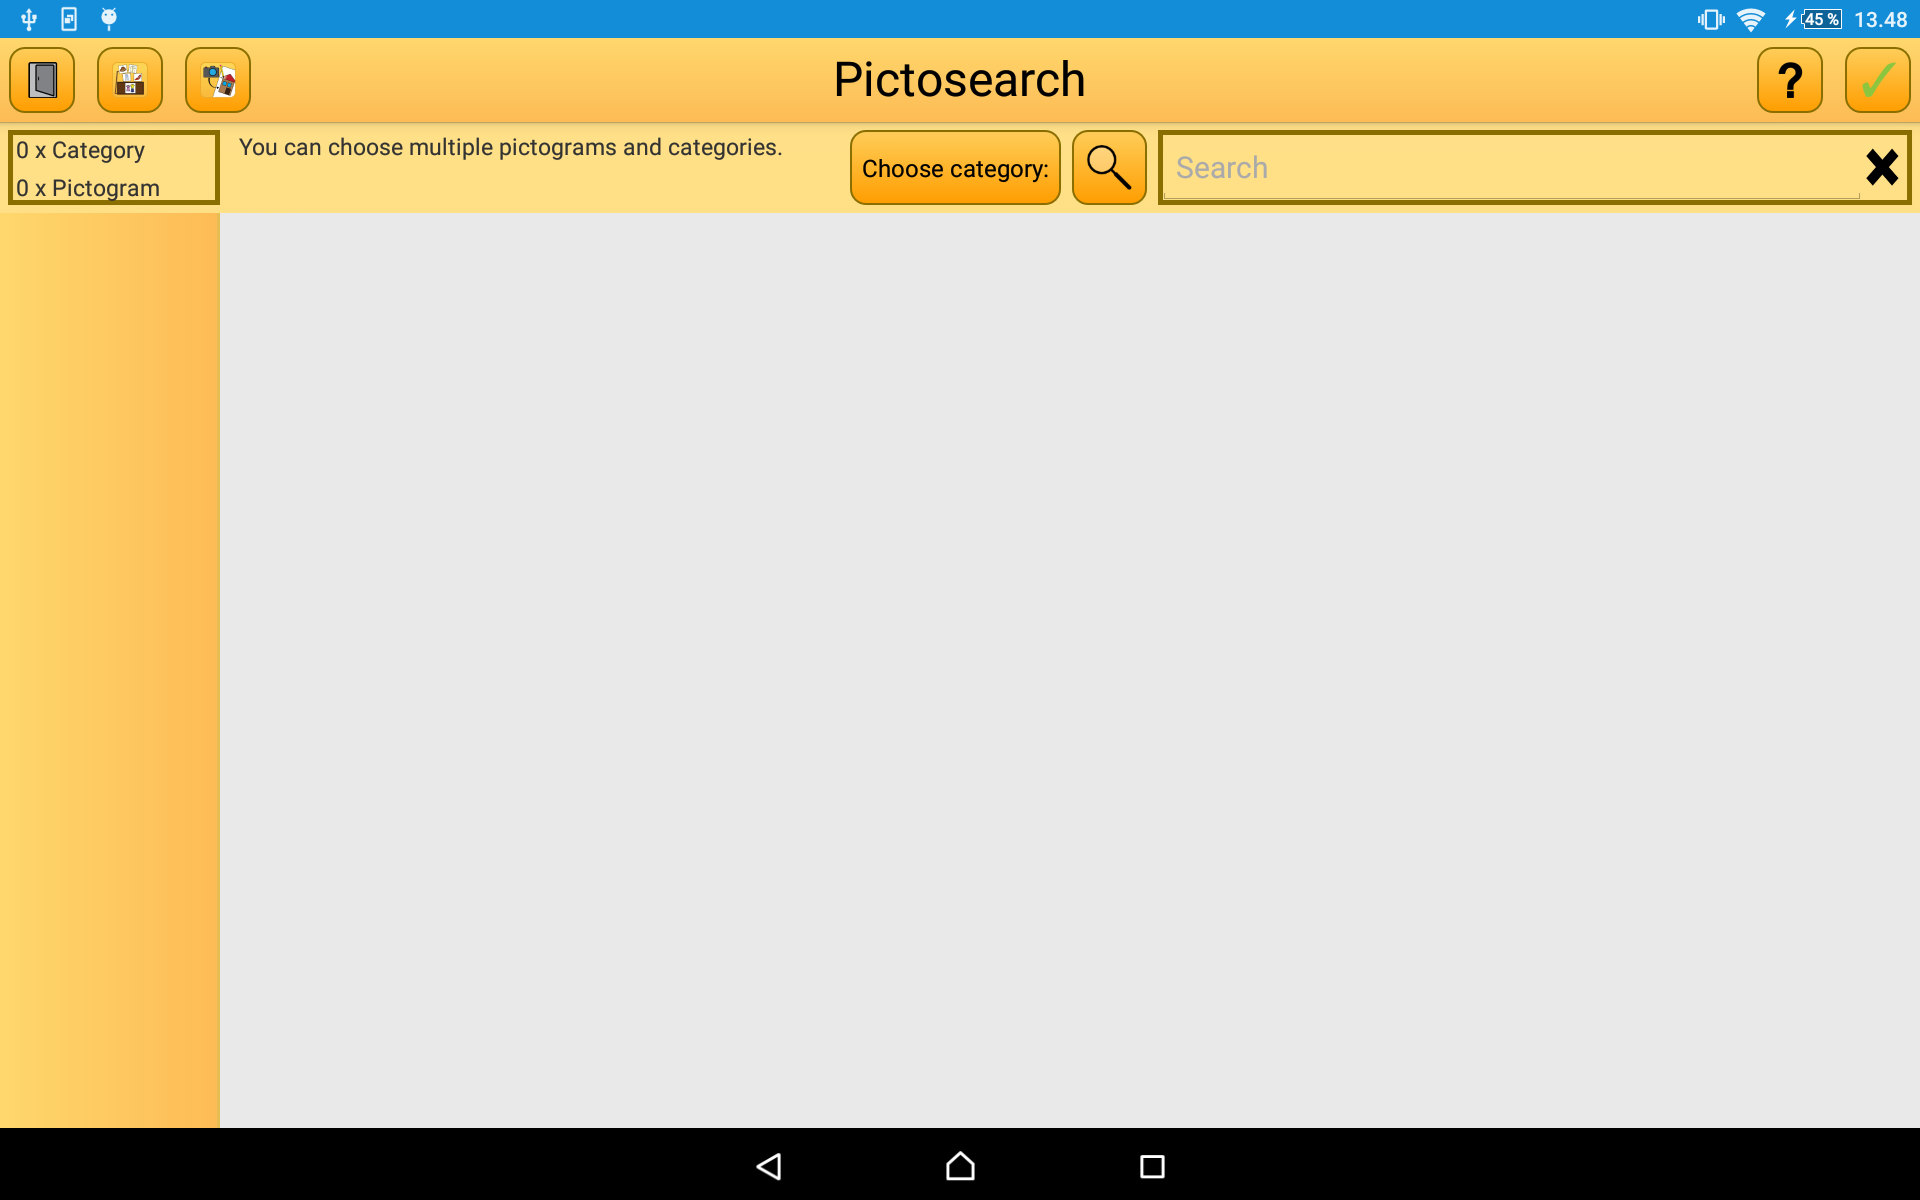
\includegraphics[width=0.8\textwidth]{images/old_startup.png}
                \end{figure}
                }

                \only<2>{
                New view:
                \begin{figure}[htb]
                    \centering
                    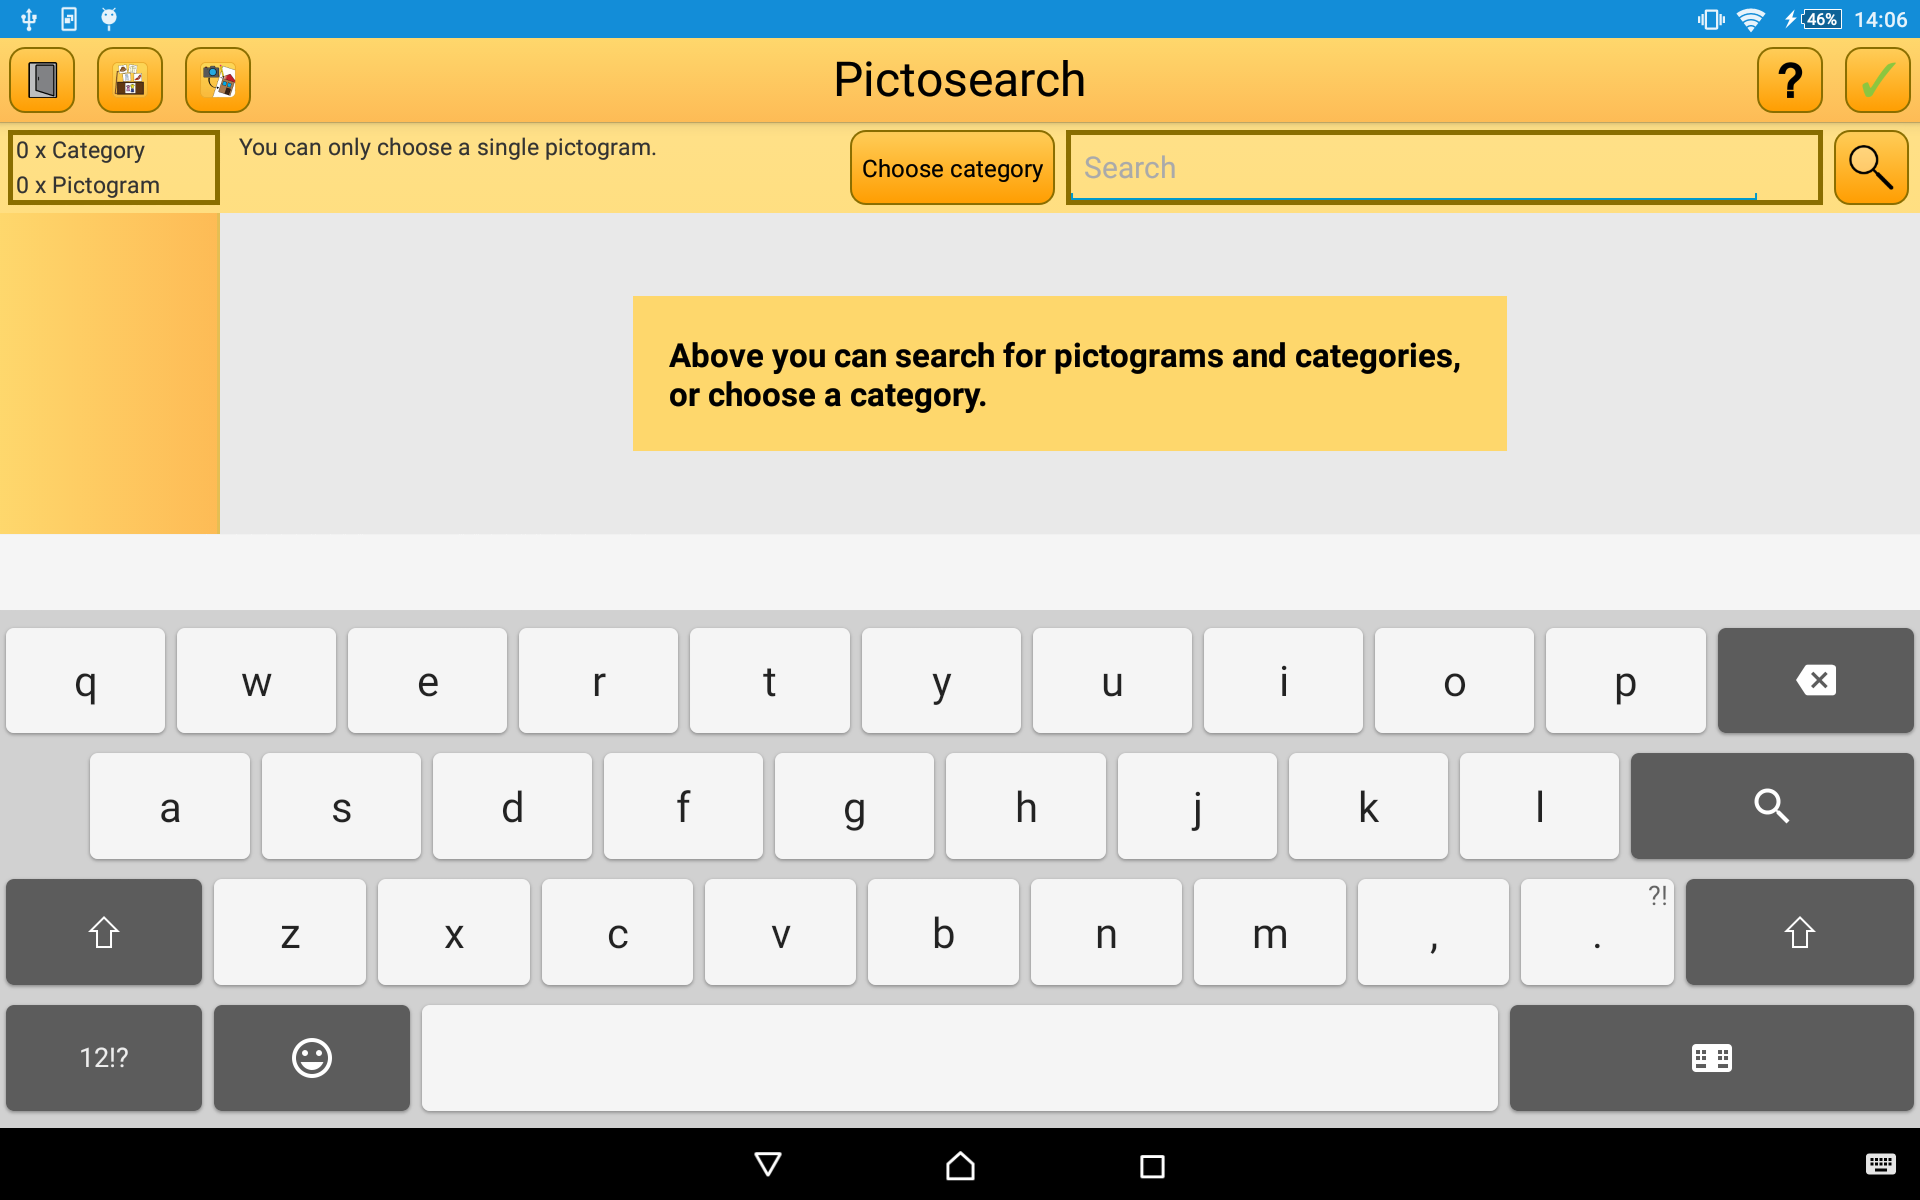
\includegraphics[width=0.8\textwidth]{images/new_startup.png}
                \end{figure}
                }

                \only<3>{
                New view after pressing a button:
                \begin{figure}[htb]
                    \centering
                    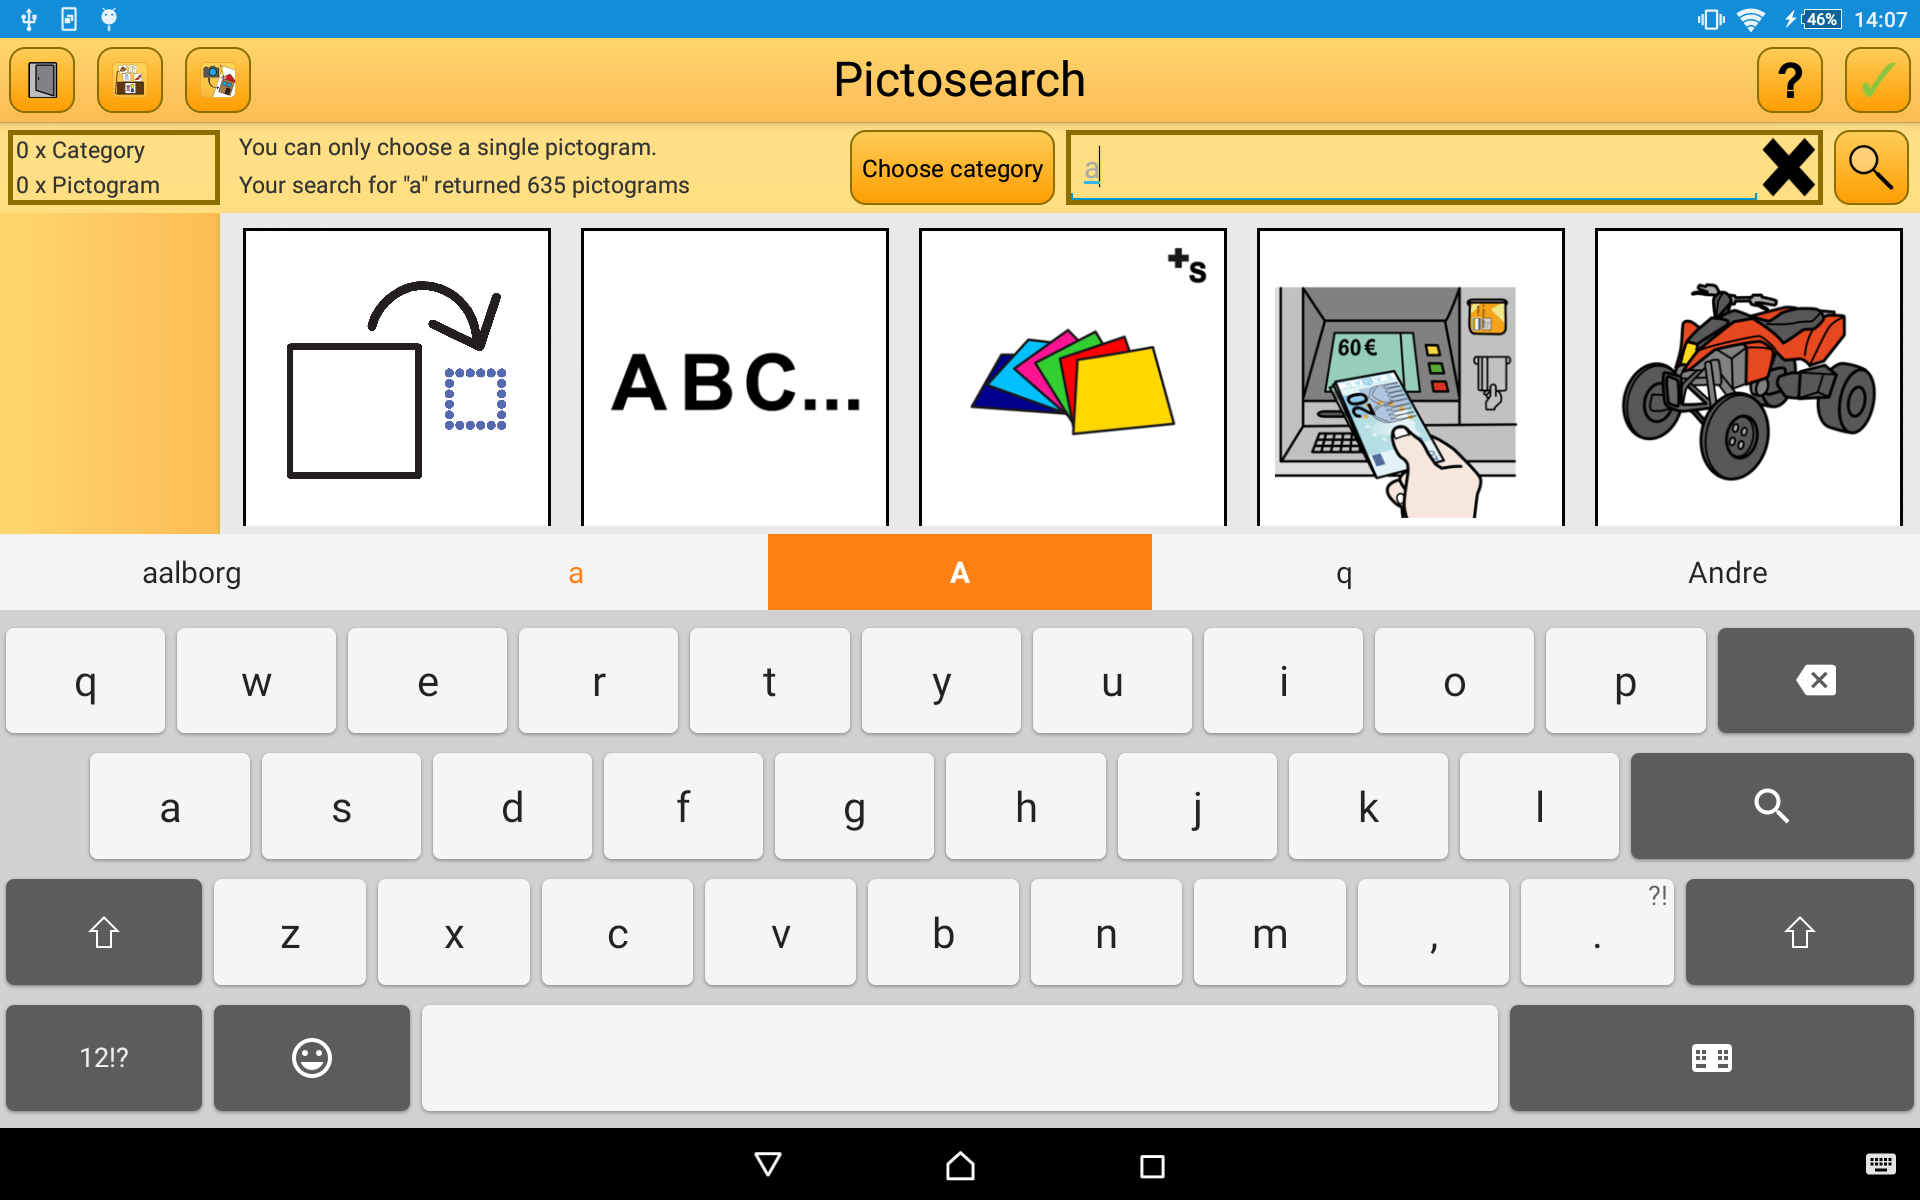
\includegraphics[width=0.8\textwidth]{images/new_searchresult.png}
                \end{figure}
                }
            \end{frame}

        \subsubsection{Week Schedule}
            \begin{frame}[t]{GIRAF--Apps}\framesubtitle{Week Schedule}
                \begin{itemize}
                    \item Added border to each frame.
                    \item Made the entire area scrollable.
                \end{itemize}
                \bigskip
                \only<1>{
                Week Schedule example:
                \begin{figure}[htb]
                    \centering
                    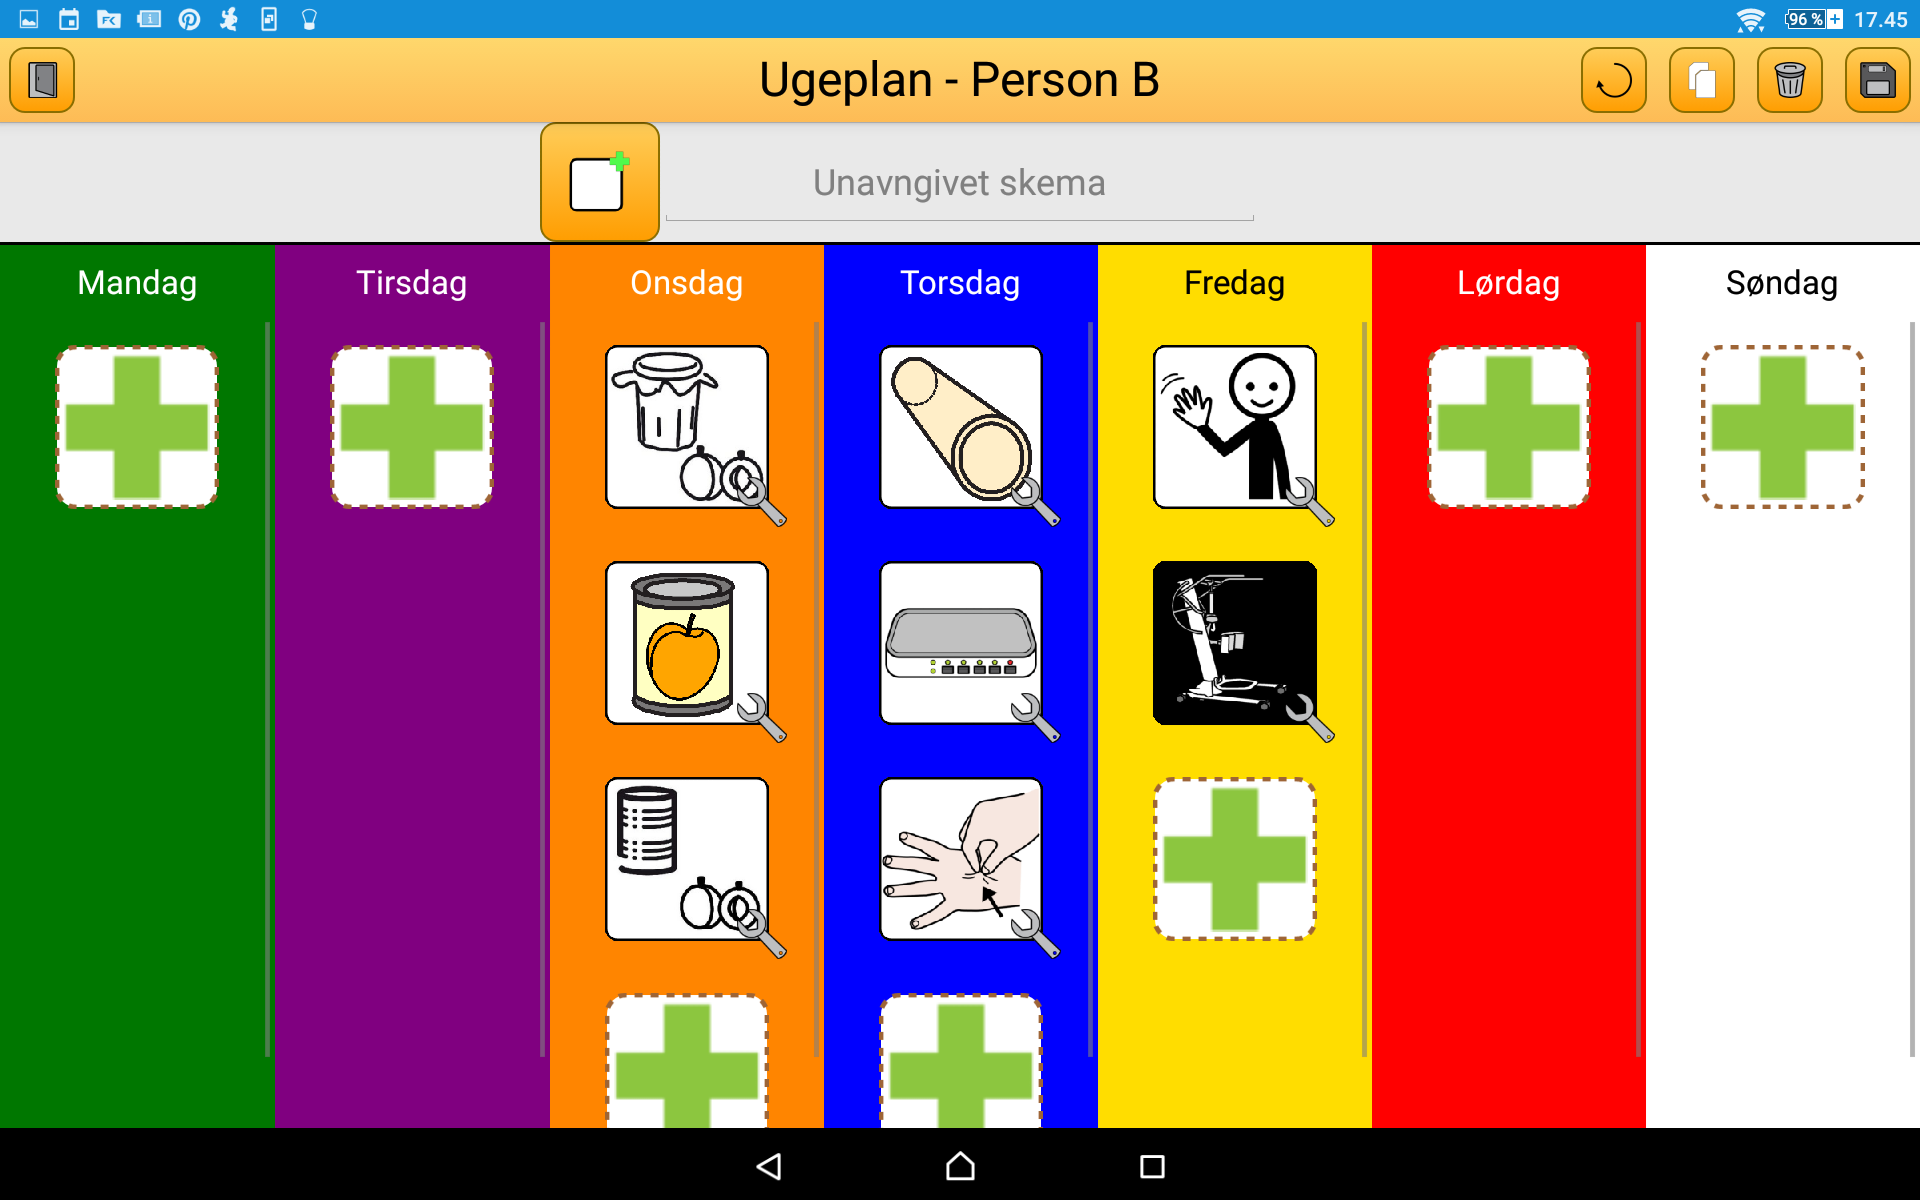
\includegraphics[width=0.8\textwidth]{images/ws_uden.png}
                \end{figure}
                }

                \only<2>{
                Week Schedule example with layoutborders:
                \begin{figure}[htb]
                    \centering
                    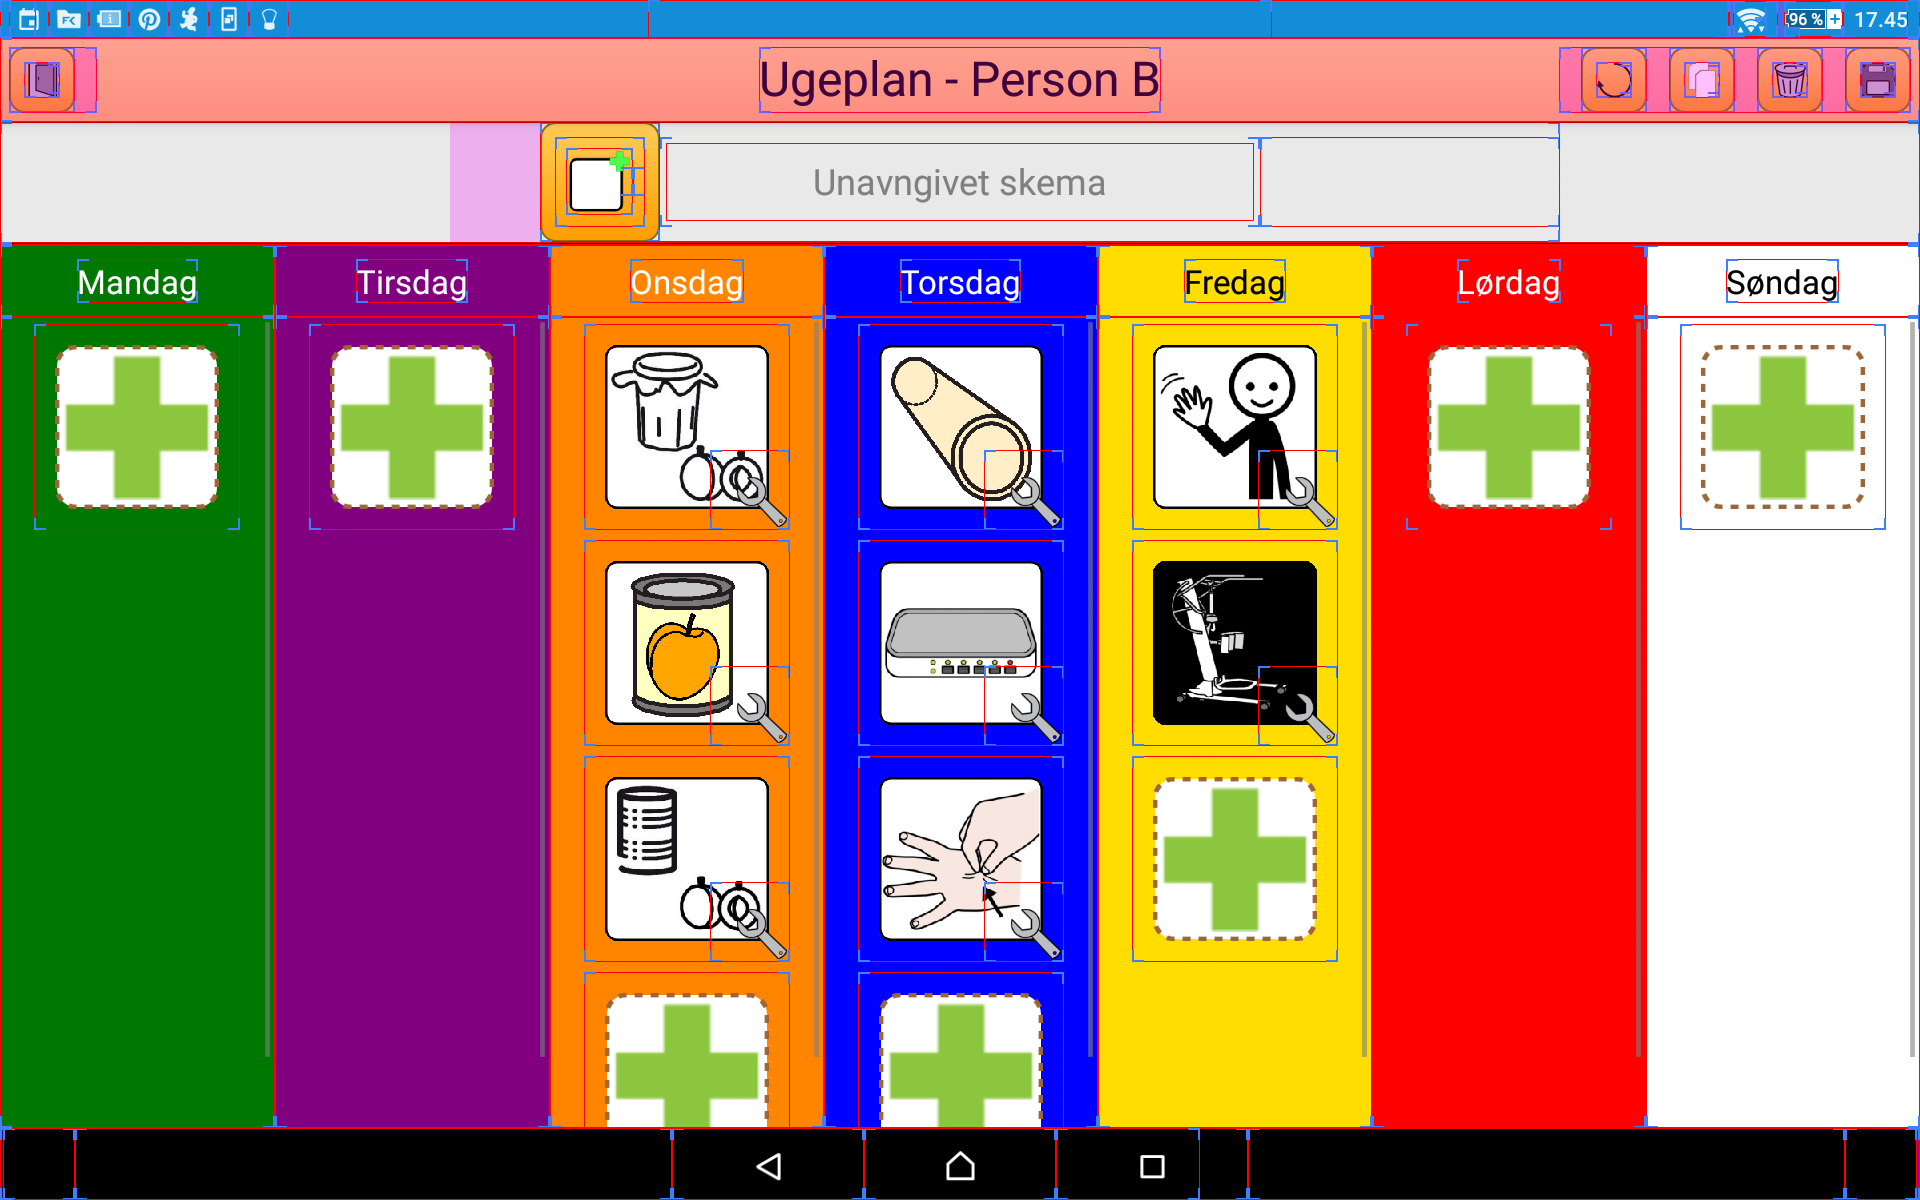
\includegraphics[width=0.8\textwidth]{images/ws_med.png}
                \end{figure}
                }


                \only<3>{
                Week Schedule example with layoutborders zoomed:
                \begin{figure}[htb]
                    \centering
                    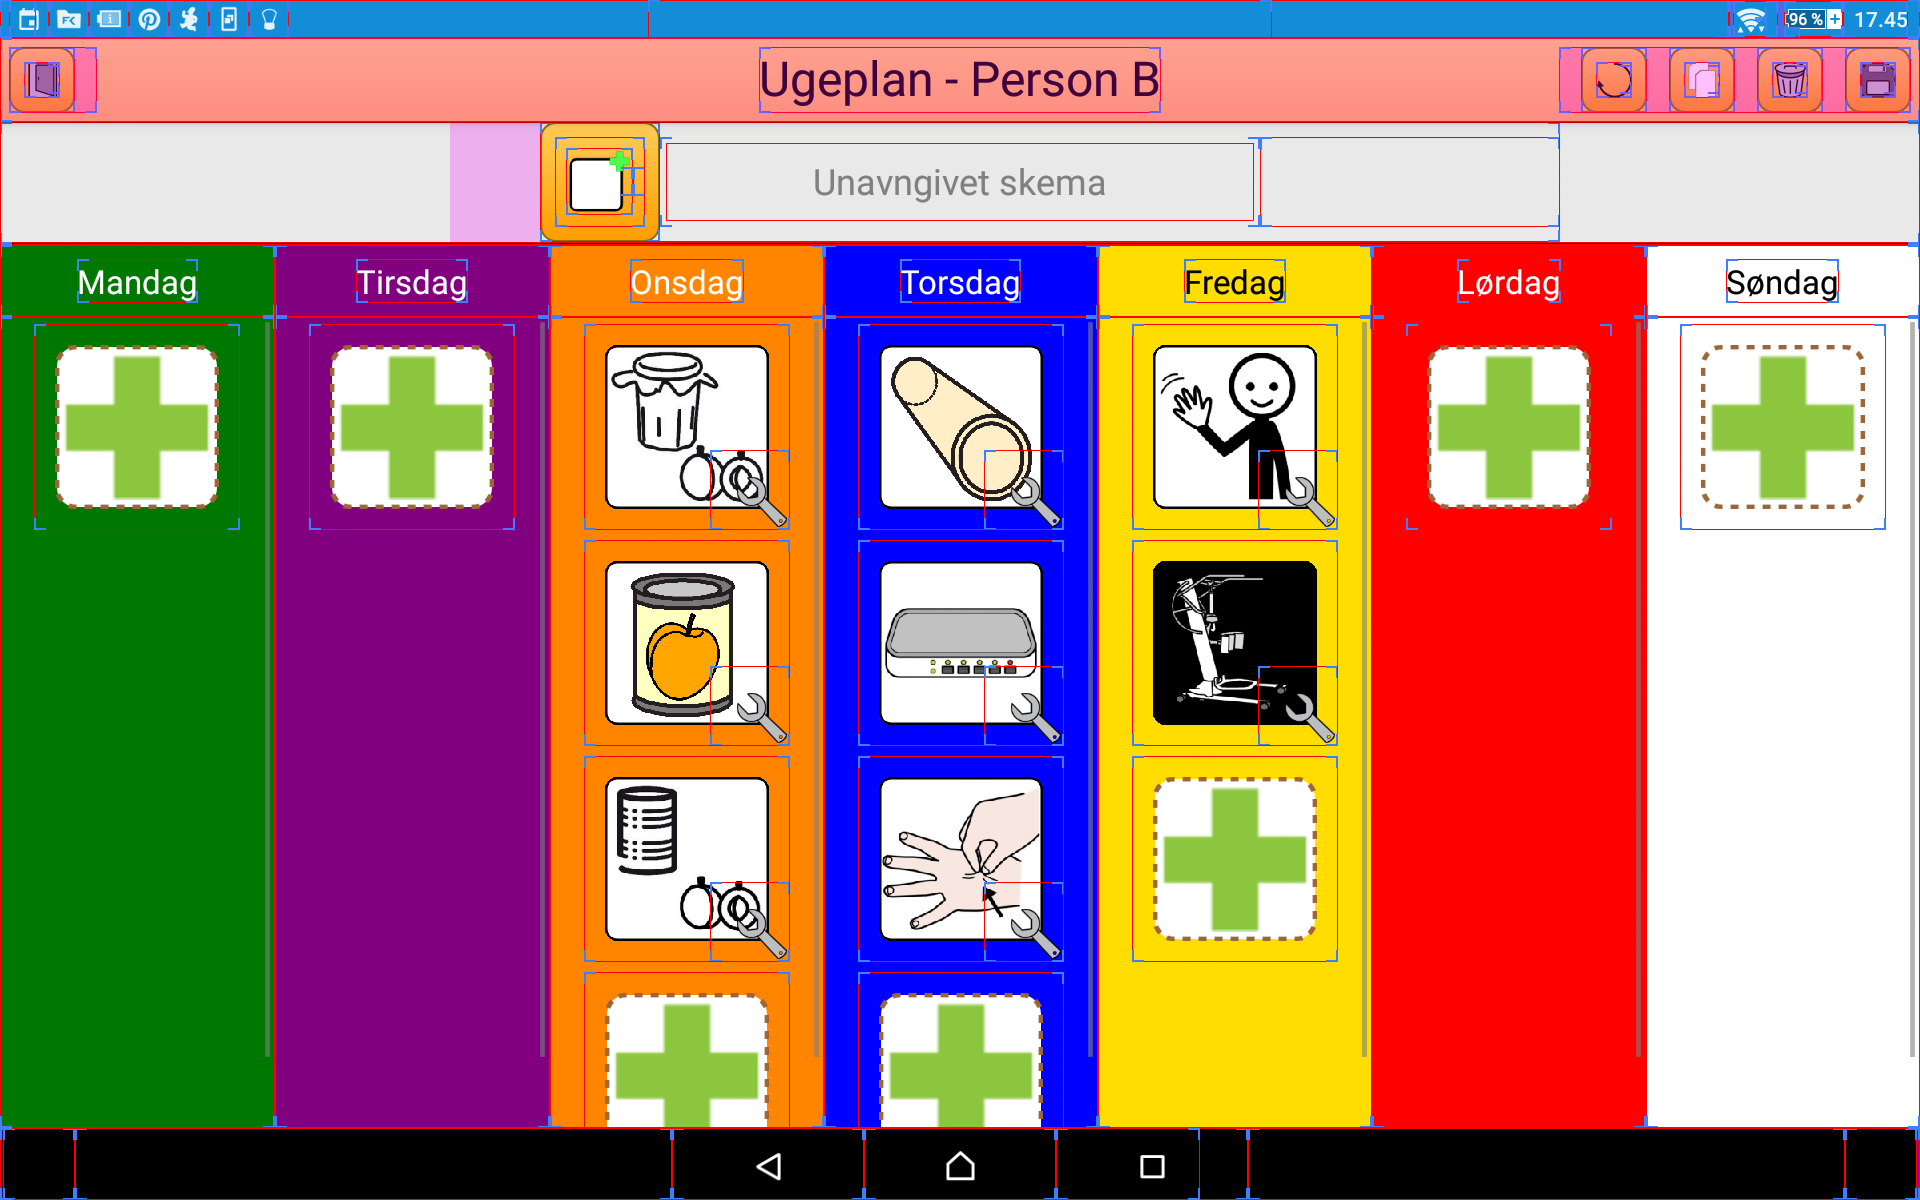
\includegraphics[trim={20cm 15.5cm 20cm 8.5cm},clip, width=0.8\textwidth]{images/ws_med.png}
                \end{figure}
                }

            \end{frame}

\section{Epilogue}
    \begin{frame}[t]{Epilogue}\framesubtitle{Content Overview}
        \begin{itemize}
            \item Multiproject Process
            \begin{itemize}
                \item Work Partitioning
                \item Areas of Responsibility
                \item REST Specific Workflow
            \end{itemize}
            \item Future Work
            \begin{itemize}
                \item Remaining Design for REST
                \item Utilising REST API
            \end{itemize}
        \end{itemize}
    \end{frame}

    \begin{frame}[t]{Multiproject Process}\framesubtitle{Work Partioning}  
        \begin{itemize}
            \item No ``experts'' on any apps
            \item Several abandoned tasks per sprint
            \item Random High Priority Selection
            \item Priority Designation
            \item Greater Focus on Cross Group Communication
        \end{itemize}
    \end{frame}

    \begin{frame}[t]{Multiproject Process}\framesubtitle{Areas of Responsibility}
        \begin{itemize}
            \item Several Perceptions
            \item More Valuable Areas of Responsibility
            \item Remove Restrictions
        \end{itemize}
    \end{frame}

    \begin{frame}[t]{Multiproject Process}\framesubtitle{REST Workflow Inspirations}
        \begin{itemize}
            \item Code-Review
            \item Linter
            \item Tests
            \item Do It Right, Not Fast
        \end{itemize}
    \end{frame}

    \begin{frame}[t]{Future Work}\framesubtitle{Future Work for the REST API}
        \begin{itemize}            
            \item More Endpoints
            \item Standalone Requirements
            \item Web Administration
            \item Client-Side Implementation
            \begin{itemize}
                \item Refactor Model
                \item Translate Data
            \end{itemize}
        \end{itemize}
    \end{frame}

    \begin{frame}[t]{}\framesubtitle{}
        \begin{itemize}
        \end{itemize}
    \end{frame}


% ====================================================

% Final slide
{\aauwavesbg
  \begin{frame}[plain,noframenumbering]
    \finalpage{\texttt{throw new PresentationIsOverException();}}
  \end{frame}}

\end{document}
